\iffalse
\let\negmedspace\undefined
\let\negthickspace\undefined
\documentclass[journal,12pt,twocolumn]{IEEEtran}
\usepackage{cite}
\usepackage{amsmath,amssymb,amsfonts,amsthm}
\usepackage{algorithmic}
\usepackage{graphicx}
\usepackage{textcomp}
\usepackage{xcolor}
\usepackage{txfonts}
\usepackage{listings}
\usepackage{enumitem}
\usepackage{mathtools}
\usepackage{gensymb}
\usepackage[breaklinks=true]{hyperref}
\usepackage{tkz-euclide} % loads  TikZ and tkz-base
\usepackage{listings}
\usepackage{gvv}


\newtheorem{theorem}{Theorem}[section]
\newtheorem{problem}{Problem}
\newtheorem{proposition}{Proposition}[section]
\newtheorem{lemma}{Lemma}[section]
\newtheorem{corollary}[theorem]{Corollary}
\newtheorem{example}{Example}[section]
\newtheorem{definition}[problem]{Definition}

\newcommand{\BEQA}{\begin{eqnarray}}
\newcommand{\EEQA}{\end{eqnarray}}
\newcommand{\define}{\stackrel{\triangle}{=}}
\theoremstyle{remark}
\newtheorem{rem}{Remark}

\graphicspath{./figs/}

%\bibliographystyle{ieeetr}
\begin{document}
%

\bibliographystyle{IEEEtran}


\vspace{3cm}

\title{
	%	\logo{
	Assignment-1 

	\large{EE:1205 Signals and Systems}

	Indian Institute of Technology, Hyderabad
	%	}
}
\author{Kunal Thorawade

EE23BTECH11035
}	

\maketitle


\newpage

%\tableofcontents

\bigskip
 
 \renewcommand{\thefigure}{\theenumi}
 \renewcommand{\thetable}{\theenumi}
 %\renewcommand{\theequation}{\theenumi}

 \section{\Large Question:}  Ramkali saved Rs 5 in the first week of a year and then increased her weekly savings by Rs 1.75. If in the $n$th week, her weekly savings become Rs 20.75, find $n$.

 \section{\Large Solution:} 
 \fi
 \begin{table}[ht]
    \centering
    \begin{tabular}{|c|c|c|}
        \hline
        Parameter & Value & Description \\
        \hline
        $x(0)$ & 5 & First term of AP \\
        $d$ & 1.75 & Common difference of AP \\
        $x(n)$ & 20.75 & $n^{th}$ term of AP \\
        \hline
    \end{tabular}
    \vspace{2mm}
    \caption{Parameter List}
    \label{tab:simple.10.5.2.20}
\end{table}


 \begin{align} 
	 x(n) &= x(0) + (n)(d)
	 \\ 20.75 &= 5 + (n)(1.75)  
	 \\ \implies 15.75 &= (n)(1.75)
	 \\ \implies n &= \frac{15.75}{1.75}
	 \\ \implies n &= 9
	 \\x(n) &= 5u(n) + 1.75nu(n)
 \end{align}
 The Z-transform of a sequence $x(n)$ is given by:
 \begin{align}
	  X(z) &= \frac{5z^{-1}}{1-z^{-1}}+\frac{1.75z^{-1}}{(1-z^{-1})^{2}} ; |z| > 1
 \end{align}

 \begin{figure}
	     \centering
	         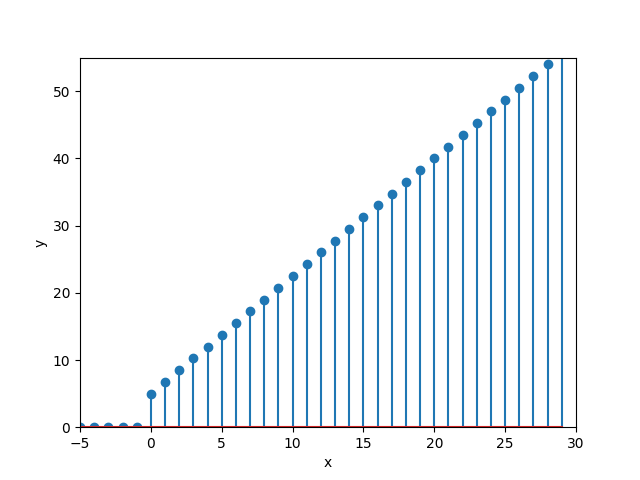
\includegraphics[width = 8cm]{ncert-maths/10/5/2/20/figs/fig1.png}
		     \caption{Plot of $x(n) = 5 + 1.75n$}
		         \label{fig:enter-label}
 \end{figure}

